\documentclass[11pt]{beamer}
\usepackage{amssymb, amsmath, url,bm}
\usepackage{graphicx}
\usepackage{mathtools}
\title{\\Coloring Gaussian Curvature on Quartic Triangular B\'ezier Patches\\ From Smooth Approximations of Irregular Closed Blender Meshes\vspace{-0.05in}}
\author{Brandon Drumheller, Adam Freeman}
\date{\vspace{-0.25in}May 19, 2016}

\begin{document}
	\begin{frame}
		\titlepage
	\end{frame}
	\vspace{-0.2in}
	\begin{frame}
		\frametitle{Project Description} 
		The goal of this project was to color Gaussian curvature on quartic triangular B\'ezier Patches. These patches were generated from smooth approximations of arbitrary closed meshes, created in the open source modeling program Blender. The refinement process follows the algorithm detailed by Loop\footnotemark.
		\footnotetext[1]{ Charles Loop. Smooth spline surfaces over irregular meshes. \textit{In Proceedings of the 21st annual conference on Computer graphics and interactive techniques}, pages 303–310. ACM, 1994.}
	\end{frame} 


	\begin{frame}
			\frametitle{Spline Construction:}
			\vspace{-0.1in}
			The spline construction is split into three stages:
			\begin{enumerate}
				\item Mesh Refinement
				\item Quad-Net Construction
				\item Quartic Triangular B\`ezier Patch Construction
			\end{enumerate}
	\vspace{0.25in}
	The output of this algorithm is a collection of quartic triangular B\`ezier patches.
	\end{frame}

	\begin{frame}
		\frametitle{Mesh Refinement - Cube}
		\vspace{-0.1in}
		The refined meshes are a ``smoothing" of the the inputted closed meshes. The meshes resulting from this step have the property that each vertex in the mesh has exactly 4 edges incident on it. As the process is computationally expensive for complex meshes simpler meshes are included for illustration.	
		\begin{figure}
			\centering
			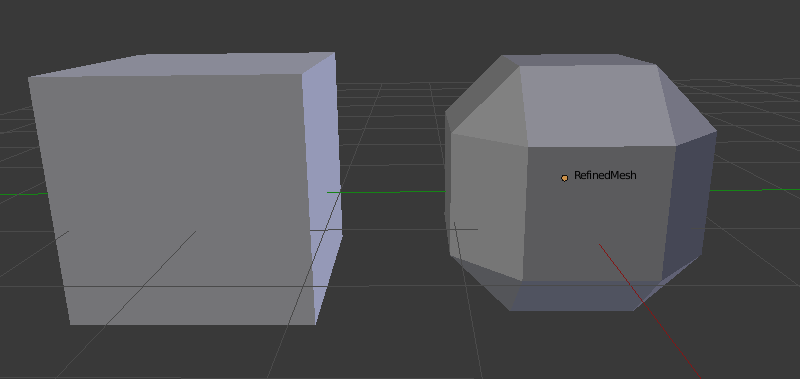
\includegraphics[width=.7\linewidth]{img/refine_cube}
						\caption{A cube (left) and the resulting refined mesh $\mathcal{M}^1$ (right).}
		\end{figure}
	\end{frame}

	\begin{frame}
		\begin{figure}
			\frametitle{Mesh Refinement - Icosphere}
			\centering
			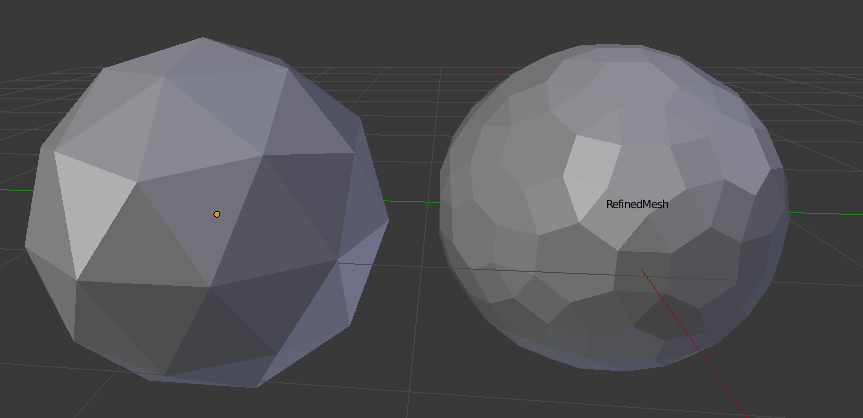
\includegraphics[width=.7\linewidth]{img/refine_icosphere}
			\caption{An icosphere (left) and the resulting refined mesh $\mathcal{M}^1$ (right).}		
		\end{figure}
	\end{frame}

	\begin{frame}
		\begin{figure}
			\frametitle{Mesh Refinement - Monkey}
			\centering
			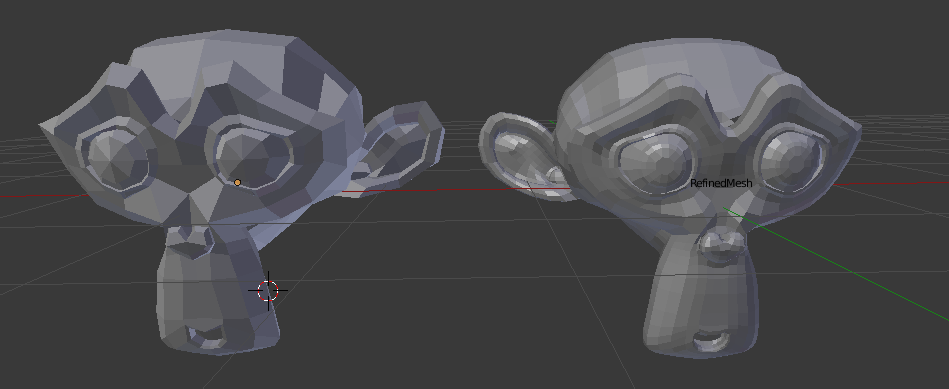
\includegraphics[width=.7\linewidth]{img/refine_monkey}
			\caption{A monkey head (nicknamed `Suzanne' left) and the resulting refined mesh $\mathcal{M}^1$ (right).}			
		\end{figure}
	\end{frame}

	\begin{frame}
		\frametitle{Quad-Net Construction}
		Quad-nets are sets of 16 points that surround each vertex. These points form nets that when ``stitched" together cover the entire refined mesh $\mathcal{M}^1$. 
	
		\begin{figure}[bp!]
			\centering			
			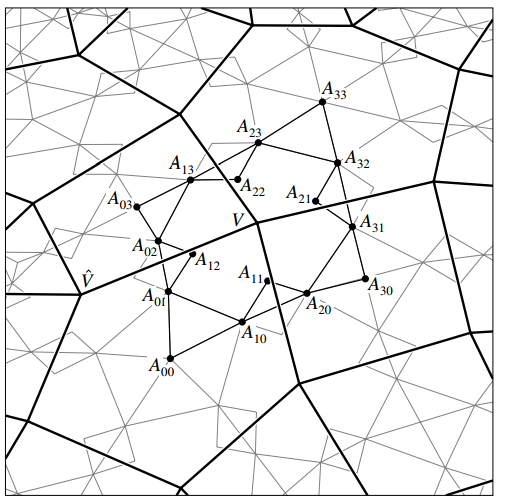
\includegraphics[width=.5\linewidth]{img/loop_quad_net}
			\caption{The quadnet corresponding to vertex $V$ on the refined mesh $\mathcal{M}^1$ [Loop 1994].}			
		\end{figure} 	
	\end{frame}

	\begin{frame}
		\begin{figure}[bp!]
			\frametitle{Quad-Net Construction - Cube}
			\centering
			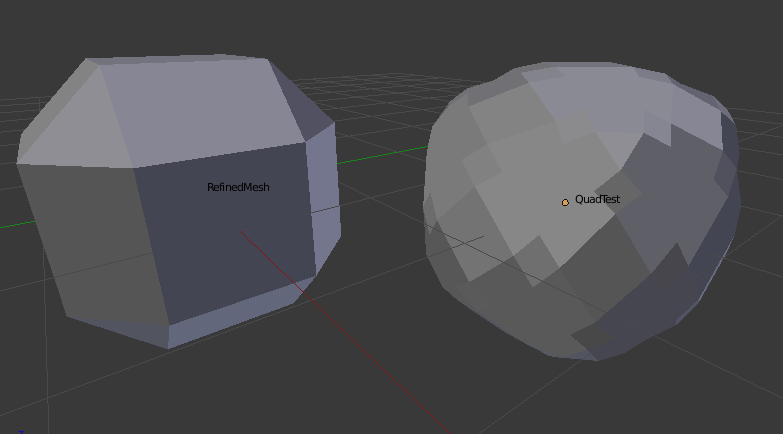
\includegraphics[width=.8\linewidth]{img/quad_cube}
			\caption{Quad-nets (right) corresponding to the cube's $\mathcal{M}^1$ (left)}	
		\end{figure}
	\end{frame}	

	\begin{frame}
		\begin{figure}[h]
			\frametitle{Quad-Net Construction - Icosphere}
			\centering
			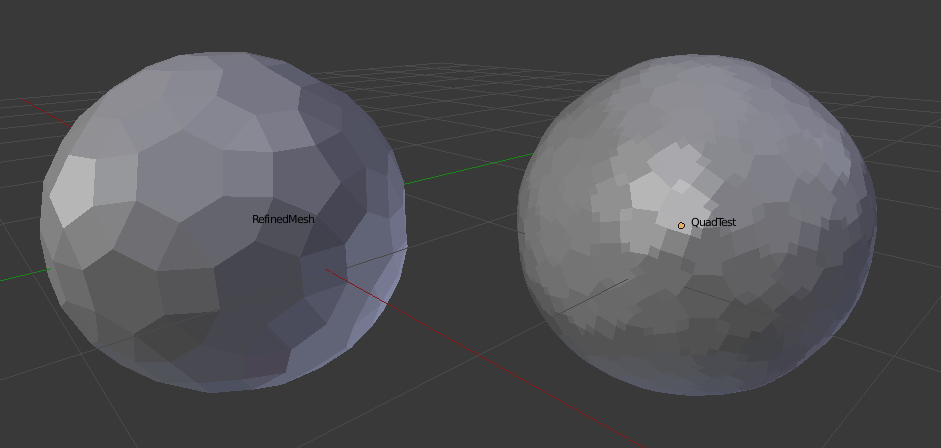
\includegraphics[width=.8\linewidth]{img/quad_icosphere}
			\caption{Quad-nets (right) corresponding to the icosphere's $\mathcal{M}^1$ (left)}	
		\end{figure}
	\end{frame}

	\begin{frame}
		\frametitle{Quad-Net Construction - Closed Mesh Restriction}
		The implementation is contingent on the fact that the $\mathcal{M}^0$ is a closed mesh. Upon closer examination one finds that the monkey head `Suzanne' is an open mesh. Although the smoothing process succeeds, quad-net resolution fails for this open surface. \\
		\begin{figure}[h]
			\centering
			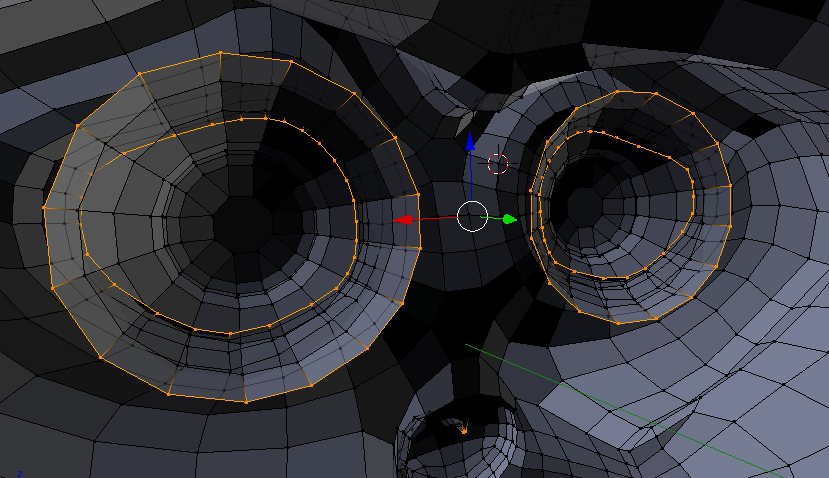
\includegraphics[width=.5\linewidth]{img/quad_monkey}
			\caption{Inside of `Suzanne'. Upon close examination one recognizes the mesh is open.}	
		\end{figure}
	\end{frame}
	

	\begin{frame}
		\frametitle{Quartic Triangular B\`ezier Patch Construction}
		The final step of the construction creates a collection of triangular patch control points, from which unique equations for quartic triangular B\`ezier patches are calculated. From these patches the Gaussian curvature is calculated and colored.   
		
		\vspace{0.25in}
		Quartic triangular B\`ezier patches are calculated using the equation ($n=4$): 
		$$\bm{\sigma}(s,t,u) = \displaystyle \sum_{\begin{smallmatrix} i+j+k=n \\ i,j,k \ge 0\end{smallmatrix}} \frac{n!}{i!j!k!} s^i t^j u^k \alpha^i \beta^j \gamma^k \quad s + t + u = 1, 0 \le s,t,u$$ 
	\end{frame}

	\begin{frame}
		\frametitle{Quartic Triangular B\`ezier Patches}
		\begin{figure}[h]
			\centering
			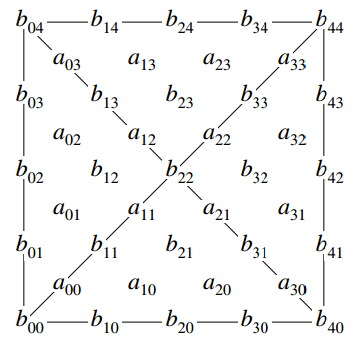
\includegraphics[width=.4\linewidth]{img/bezier_loop}
			\caption{The 4 triangular B\`ezier patches on a quad-net. [Loop 1994]}	
		\end{figure}
	\end{frame}	

	\begin{frame}
		\begin{figure}[h]
			\frametitle{Quartic Triangular B\`ezier Patches}
			\centering
			\includegraphics[width=.55\linewidth]{img/quartic}
			\caption{Application of the aforementioned formula to the left triangular B\`ezier patch in the previous figure.}
		\end{figure}
	\end{frame}

	\begin{frame}
		\frametitle{Quartic Triangular B\`ezier Patches}
		One notes that the aforementioned formula is equivalently expressed in the usual $u,v$ parametrization with $n=4$ as: 
		$$\displaystyle \bm{\sigma}(u,v) = \sum_{\begin{smallmatrix} i+j+k=n \\ i,j,k \ge 0\end{smallmatrix}} \frac{n!}{i!j!k!} (1-u-v)^i u^j v^k \alpha^i \beta^j \gamma^k \quad0 \le u,v \quad u + v \le 1$$
	\end{frame}

	\begin{frame}
		\begin{figure}[h]
			\frametitle{Quartic Triangular B\`ezier Patches}
			\centering
			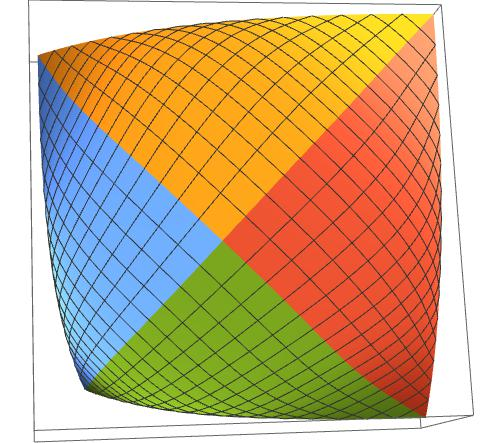
\includegraphics[width=.43\linewidth]{img/bezier_patch}
			\caption{Mathematica Plot of Quartic Triangular B\`ezier patches from  a cubic Blender mesh.}
		\end{figure}
	\end{frame}

	\begin{frame}
		\frametitle{Coloring Quartic B\`ezier Patches:}
		$\langle$add explanation of coloring process here$\rangle$
	\end{frame}

	\begin{frame}
		\frametitle{Images/animations:}
		$\langle$Add images and animations along with explanations here.$\rangle$
	\end{frame}

	
	\begin{frame}
		\centering
		\underline{{\huge Demonstration}}
	\end{frame}
	

	\begin{frame} 
		\frametitle{Software:}
		Blender, Python 3.5.1, Mathematica
	\end{frame}

	\begin{frame}
		\centering
		\underline{{\huge Questions}}
	\end{frame}
	
\end{document}